\documentclass{article}
\usepackage[T1]{fontenc}
\usepackage{lmodern}
\usepackage{graphicx}
\usepackage{amsmath,amssymb}
\usepackage[a4paper,margin=2cm]{geometry}
\usepackage[absolute,overlay]{textpos}
\setlength{\TPHorizModule}{1mm}
\setlength{\TPVertModule}{1mm}
\usepackage[indonesian]{babel}
\usepackage{hyperref}
\setlength{\emergencystretch}{2em}
% unit: Halaman 29

\begin{document}

% === Halaman 29 (python/native) ===

• Contoh lain: Kurva eliptik  y2  x3 + x + 1 (mod 23) memiliki titik-titik di dalam 

himpunan \{(0, 1), (0, 22), (1, 7), (1, 16), (3, 10), (3, 13), (5, 4), (5, 19) , (6, 4),  (6, 

19), (7,  11), (7, 12), (9, 7), (9, 16), (11, 3), (11, 20), (12, 4), (12,   19), (13, 7), (13, 

16), (17, 3), (17, 20), (18, 3), (18, 20), (19, 5), (19, 18)\}. 

29

% deskripsi: gambar native xref 125
\noindent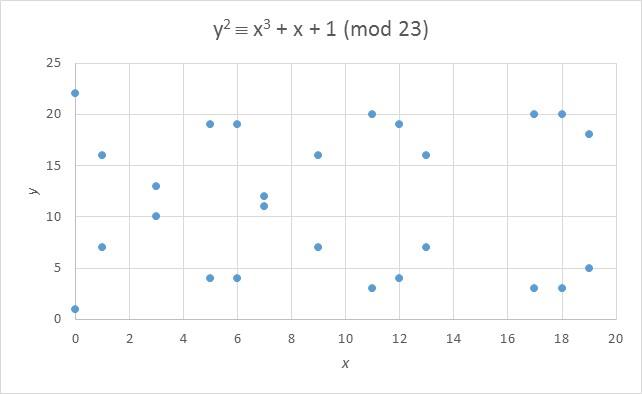
\includegraphics[width=0.85\textwidth]{../../images/python/page_029_img_01.jpeg}

\end{document}
